\documentclass{article}
\usepackage{amsmath,amssymb}
\usepackage{graphicx}
\usepackage{enumerate}
\usepackage{hyperref}
\usepackage{subcaption}
\usepackage{caption}
\usepackage{xcolor}
\usepackage{float}

\pagestyle{empty} \addtolength{\textwidth}{1.0in}
\addtolength{\textheight}{0.5in}
\addtolength{\oddsidemargin}{-0.5in}
\addtolength{\evensidemargin}{-0.5in}
\newcommand{\ruleskip}{\bigskip\hrule\bigskip}
\newcommand{\nodify}[1]{{\sc #1}}
\newcommand{\points}[1]{{\textbf{[#1 points]}}}
\newcommand{\subquestionpoints}[1]{{[#1 points]}}
\newenvironment{answer}{{\bf Answer:} \sf }{}%

\newcommand{\bitem}{\begin{list}{$\bullet$}%
{\setlength{\itemsep}{0pt}\setlength{\topsep}{0pt}%
\setlength{\rightmargin}{0pt}}}
\newcommand{\eitem}{\end{list}}

\setlength{\parindent}{0pt} \setlength{\parskip}{0.5ex}
\setlength{\unitlength}{1cm}

\newcommand{\pa}[1]{[[PA: #1]]}

\renewcommand{\Re}{{\mathbb R}}
\newcommand{\E}{{\rm E}}
\begin{document}

\pagestyle{myheadings} \markboth{}{CS 294-158 Deep Unsupervised Learning, Homework 3, Spring 2020}

{\huge
\noindent Homework 3: Latent Variable Models}
\ruleskip

{\bf Deliverable}: This PDF write-up by {\bf Tuesday March 10th, 23:59pm}.  Your PDF should be generated by simply replacing the placeholder images of this LaTeX document with the appropriate solution images that will be generated automatically when solving each question. The solution images are automatically generated and saved using the accompanying IPython notebook. Your PDF is to be submitted into Gradescope. This PDF already contains a few solution images.  These images will allow you to check your own solution to ensure correctness.


\vspace{.2in}

%--------------------------------------------------------------------------------
%--------------------------------------------------------------------------------
%--------------------------------------------------------------------------------
\noindent {\bf Question 1: VAEs on 2D Data [20pt]}
%--------------------------------------------------------------------------------
%--------------------------------------------------------------------------------
%--------------------------------------------------------------------------------

\begin{enumerate}[(a)]

\item {\bf [10pt] Data from a Full Covariance Gaussian} \\\\
Final Full -ELBO: 4.4388, Recon Loss: 2.7630, KL Loss: 1.6758 (Dataset 1)
\begin{figure}[H]
    \centering
    \begin{subfigure}{0.32\textwidth}
        \centering
        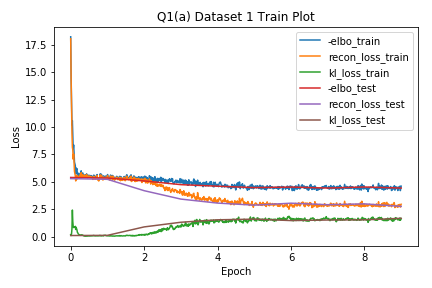
\includegraphics[width=\textwidth]{figures/q1_a_dset1_train_plot.png}
        \caption{Training curve}
    \end{subfigure}
    \begin{subfigure}{0.32\textwidth}
        \centering
        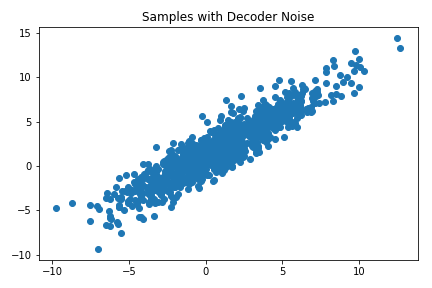
\includegraphics[width=\textwidth]{figures/q1_a_dset1_sample_with_noise.png}
        \caption{Samples with Noise}
    \end{subfigure}
    \begin{subfigure}{0.32\textwidth}
        \centering
        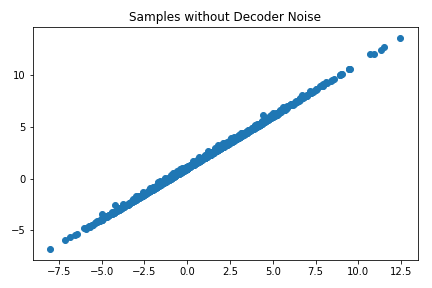
\includegraphics[width=\textwidth]{figures/q1_a_dset1_sample_without_noise.png}
        \caption{Samples without Noise}
    \end{subfigure}
    \caption{Results for Dataset 1}
\end{figure}
Final Full -ELBO: \textcolor{red}{FILL}, Recon Loss: \textcolor{red}{FILL}, KL Loss: \textcolor{red}{FILL} (Dataset 2)
\begin{figure}[H]
    \centering
    \begin{subfigure}{0.32\textwidth}
        \centering
        
\includegraphics[width=\textwidth]{figures/q1_a_dset2_train_plot.png}
        \caption{Training curve}
    \end{subfigure}
    \begin{subfigure}{0.32\textwidth}
        \centering
        
\includegraphics[width=\textwidth]{figures/q1_a_dset2_sample_with_noise.png}
        \caption{Samples with Noise}
    \end{subfigure}
    \begin{subfigure}{0.32\textwidth}
        \centering
        
\includegraphics[width=\textwidth]{figures/q1_a_dset2_sample_without_noise.png}
        \caption{Samples without Noise}
    \end{subfigure}
    \caption{Results for Dataset 2}
\end{figure}

\newpage

\item {\bf [10pt] Data from a Diagonal Gaussian} \\\\
Final Full -ELBO: 4.4213, Recon Loss: 4.4094, KL Loss: 0.0119 (Dataset 1)
\begin{figure}[H]
    \centering
    \begin{subfigure}{0.32\textwidth}
        \centering
        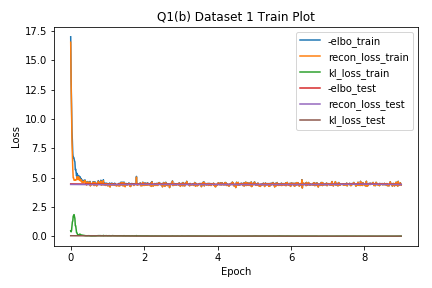
\includegraphics[width=\textwidth]{figures/q1_b_dset1_train_plot.png}
        \caption{Training curve}
    \end{subfigure}
    \begin{subfigure}{0.32\textwidth}
        \centering
        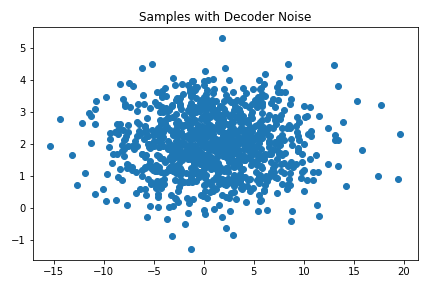
\includegraphics[width=\textwidth]{figures/q1_b_dset1_sample_with_noise.png}
        \caption{Samples with Noise}
    \end{subfigure}
    \begin{subfigure}{0.32\textwidth}
        \centering
        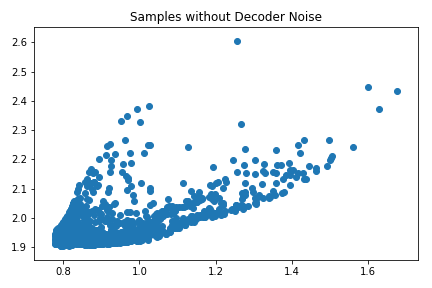
\includegraphics[width=\textwidth]{figures/q1_b_dset1_sample_without_noise.png}
        \caption{Samples without Noise}
    \end{subfigure}
    \caption{Results for Dataset 1}
\end{figure}
Final Full -ELBO: \textcolor{red}{FILL}, Recon Loss: \textcolor{red}{FILL}, KL Loss: \textcolor{red}{FILL} (Dataset 2)
\begin{figure}[H]
    \centering
    \begin{subfigure}{0.32\textwidth}
        \centering
        
\includegraphics[width=\textwidth]{figures/q1_b_dset2_train_plot.png}
        \caption{Training curve}
    \end{subfigure}
    \begin{subfigure}{0.32\textwidth}
        \centering
        
\includegraphics[width=\textwidth]{figures/q1_b_dset2_sample_with_noise.png}
        \caption{Samples with Noise}
    \end{subfigure}
    \begin{subfigure}{0.32\textwidth}
        \centering
        
\includegraphics[width=\textwidth]{figures/q1_b_dset2_sample_without_noise.png}
        \caption{Samples without Noise}
    \end{subfigure}
    \caption{Results for Dataset 2}
\end{figure}
\textbf{Answer: Your answer to the reflection portion of part (b) reflection here (replace this text)}
\end{enumerate}



%--------------------------------------------------------------------------------
%--------------------------------------------------------------------------------
%--------------------------------------------------------------------------------
\newpage
\noindent {\bf Question 2: VAEs on Images [40pt]}
%--------------------------------------------------------------------------------
%--------------------------------------------------------------------------------
%--------------------------------------------------------------------------------

\begin{enumerate}[(a)]
  \item {\bf [20pt] VAE} \\\\
  Final Full -ELBO: 104.0417, Recon Loss: 79.3798, KL Loss: 24.6620 (Dataset 1)
  \begin{figure}[H]
         \centering
         \begin{subfigure}[b]{0.475\textwidth}
             \centering
             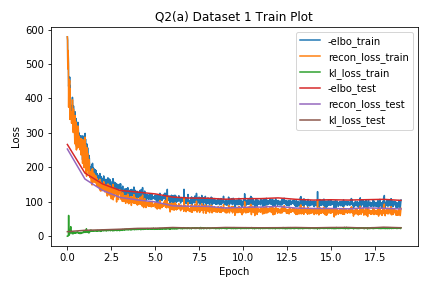
\includegraphics[width=\textwidth]{figures/q2_a_dset1_train_plot.png}
             \caption{Training Curve}
         \end{subfigure}
         \hfill
         \begin{subfigure}[b]{0.475\textwidth}
             \centering
             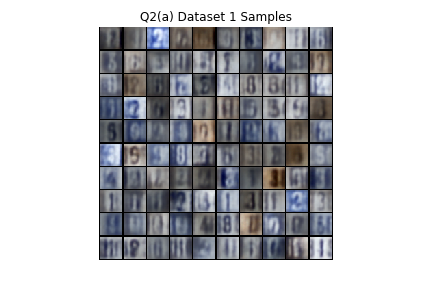
\includegraphics[width=\textwidth]{figures/q2_a_dset1_samples.png}
             \caption{Samples}
         \end{subfigure}
         \vskip\baselineskip
         \begin{subfigure}[b]{0.475\textwidth}
             \centering
             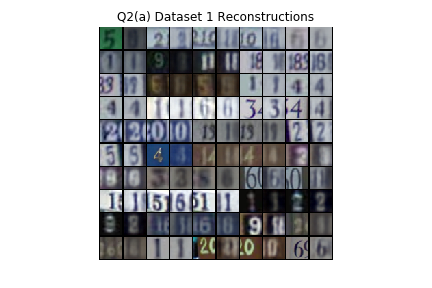
\includegraphics[width=\textwidth]{figures/q2_a_dset1_reconstructions.png}
             \caption{Reconstructions}
         \end{subfigure}
         \quad
         \begin{subfigure}[b]{0.475\textwidth}
             \centering
             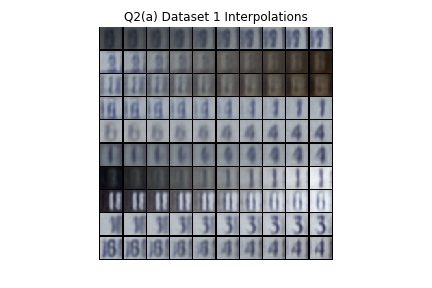
\includegraphics[width=\textwidth]{figures/q2_a_dset1_interpolations.png}
             \caption{Interpolations}
         \end{subfigure}
         \caption{Results for Dataset 1}
     \end{figure}

     \newpage

     Final Full -ELBO: \textcolor{red}{FILL}, Recon Loss: \textcolor{red}{FILL}, KL Loss: \textcolor{red}{FILL} (Dataset 2)
     \begin{figure}[H]
            \centering
            \begin{subfigure}[b]{0.475\textwidth}
                \centering
                
\includegraphics[width=\textwidth]{figures/q2_a_dset2_train_plot.png}
                \caption{Training Curve}
            \end{subfigure}
            \hfill
            \begin{subfigure}[b]{0.475\textwidth}
                \centering
                
\includegraphics[width=\textwidth]{figures/q2_a_dset2_samples.png}
                \caption{Samples}
            \end{subfigure}
            \vskip\baselineskip
            \begin{subfigure}[b]{0.475\textwidth}
                \centering
                
\includegraphics[width=\textwidth]{figures/q2_a_dset2_reconstructions.png}
                \caption{Reconstructions}
            \end{subfigure}
            \quad
            \begin{subfigure}[b]{0.475\textwidth}
                \centering
                
\includegraphics[width=\textwidth]{figures/q2_a_dset2_interpolations.png}
                \caption{Interpolations}
            \end{subfigure}
            \caption{Results for Dataset 2}
        \end{figure}

        \newpage

        \item {\bf [20pt] VAE with AF Prior} \\\\
        Final Full -ELBO: 102.5659, Recon Loss: 80.2548, KL Loss: 22.3111 (Dataset 1)
        \begin{figure}[H]
               \centering
               \begin{subfigure}[b]{0.475\textwidth}
                   \centering
                   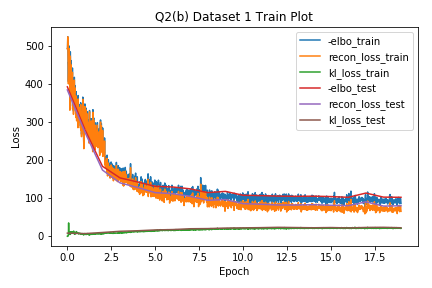
\includegraphics[width=\textwidth]{figures/q2_b_dset1_train_plot.png}
                   \caption{Training Curve}
               \end{subfigure}
               \hfill
               \begin{subfigure}[b]{0.475\textwidth}
                   \centering
                   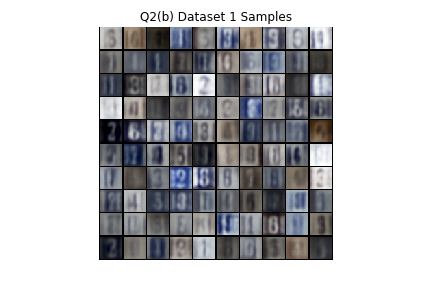
\includegraphics[width=\textwidth]{figures/q2_b_dset1_samples.png}
                   \caption{Samples}
               \end{subfigure}
               \vskip\baselineskip
               \begin{subfigure}[b]{0.475\textwidth}
                   \centering
                   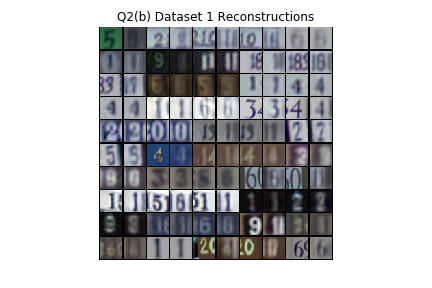
\includegraphics[width=\textwidth]{figures/q2_b_dset1_reconstructions.png}
                   \caption{Reconstructions}
               \end{subfigure}
               \quad
               \begin{subfigure}[b]{0.475\textwidth}
                   \centering
                   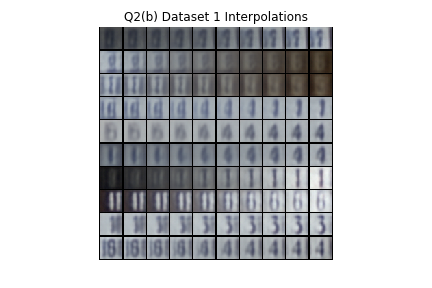
\includegraphics[width=\textwidth]{figures/q2_b_dset1_interpolations.png}
                   \caption{Interpolations}
               \end{subfigure}
               \caption{Results for Dataset 1}
           \end{figure}

           \newpage

           Final Full -ELBO: \textcolor{red}{FILL}, Recon Loss: \textcolor{red}{FILL}, KL Loss: \textcolor{red}{FILL} (Dataset 2)
           \begin{figure}[H]
                  \centering
                  \begin{subfigure}[b]{0.475\textwidth}
                      \centering
                      
\includegraphics[width=\textwidth]{figures/q2_b_dset2_train_plot.png}
                      \caption{Training Curve}
                  \end{subfigure}
                  \hfill
                  \begin{subfigure}[b]{0.475\textwidth}
                      \centering
                      
\includegraphics[width=\textwidth]{figures/q2_b_dset2_samples.png}
                      \caption{Samples}
                  \end{subfigure}
                  \vskip\baselineskip
                  \begin{subfigure}[b]{0.475\textwidth}
                      \centering
                      
\includegraphics[width=\textwidth]{figures/q2_b_dset2_reconstructions.png}
                      \caption{Reconstructions}
                  \end{subfigure}
                  \quad
                  \begin{subfigure}[b]{0.475\textwidth}
                      \centering
                      
\includegraphics[width=\textwidth]{figures/q2_b_dset2_interpolations.png}
                      \caption{Interpolations}
                  \end{subfigure}
                  \caption{Results for Dataset 2}
              \end{figure}
\end{enumerate}

%--------------------------------------------------------------------------------
%--------------------------------------------------------------------------------
%--------------------------------------------------------------------------------
\newpage
\noindent {\bf Question 3: VQ-VAE [40pt]}
%--------------------------------------------------------------------------------
%--------------------------------------------------------------------------------
%--------------------------------------------------------------------------------

Final VQ-VAE Test Loss: 0.0286, PixelCNN Prior Test Los: 1.9440 (Dataset 1)
\begin{figure}[H]
       \centering
       \begin{subfigure}[b]{0.475\textwidth}
           \centering
           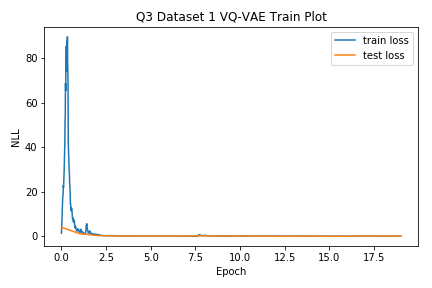
\includegraphics[width=\textwidth]{figures/q3_dset1_vqvae_train_plot.png}
           \caption{VQ-VAE Training Curve}
       \end{subfigure}
       \hfill
       \begin{subfigure}[b]{0.475\textwidth}
           \centering
           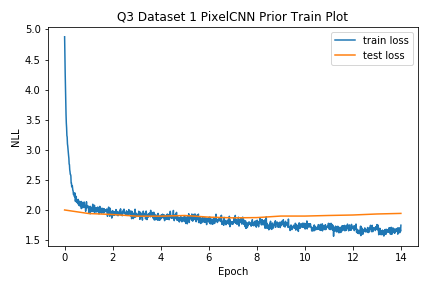
\includegraphics[width=\textwidth]{figures/q3_dset1_pixelcnn_train_plot.png}
           \caption{PixelCNN Prior Training Curve}
       \end{subfigure}
       \vskip\baselineskip
       \begin{subfigure}[b]{0.475\textwidth}
           \centering
           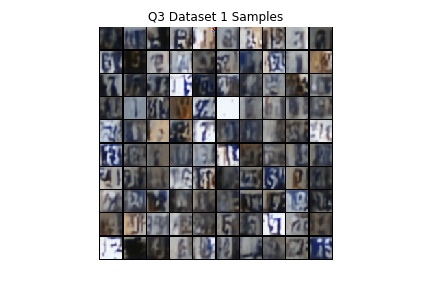
\includegraphics[width=\textwidth]{figures/q3_dset1_samples.png}
           \caption{Samples}
       \end{subfigure}
       \quad
       \begin{subfigure}[b]{0.475\textwidth}
           \centering
           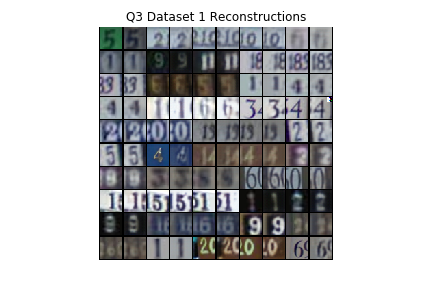
\includegraphics[width=\textwidth]{figures/q3_dset1_reconstructions.png}
           \caption{Reconstructions}
       \end{subfigure}
       \caption{Results for Dataset 1}
   \end{figure}

   \newpage

   Final VQ-VAE Test Loss: \textcolor{red}{FILL}, PixelCNN Prior Test Los: \textcolor{red}{FILL} (Dataset 2)
   \begin{figure}[H]
          \centering
          \begin{subfigure}[b]{0.475\textwidth}
              \centering
              
\includegraphics[width=\textwidth]{figures/q3_dset2_vqvae_train_plot.png}
              \caption{VQ-VAE Training Curve}
          \end{subfigure}
          \hfill
          \begin{subfigure}[b]{0.475\textwidth}
              \centering
              
\includegraphics[width=\textwidth]{figures/q3_dset2_pixelcnn_train_plot.png}
              \caption{PixelCNN Prior Training Curve}
          \end{subfigure}
          \vskip\baselineskip
          \begin{subfigure}[b]{0.475\textwidth}
              \centering
              
\includegraphics[width=\textwidth]{figures/q3_dset2_samples.png}
              \caption{Samples}
          \end{subfigure}
          \quad
          \begin{subfigure}[b]{0.475\textwidth}
              \centering
              
\includegraphics[width=\textwidth]{figures/q3_dset2_reconstructions.png}
              \caption{Reconstructions}
          \end{subfigure}
          \caption{Results for Dataset 1}
      \end{figure}

%--------------------------------------------------------------------------------
%--------------------------------------------------------------------------------
%--------------------------------------------------------------------------------
\newpage
\noindent {\bf Question 4: Bonus [15pt]}
%--------------------------------------------------------------------------------
%--------------------------------------------------------------------------------
%--------------------------------------------------------------------------------
\begin{enumerate}
    \item {\bf [10pt] Improving VQ-VAE Results} \\\\
    Final VQ-VAE Test Loss: \textcolor{red}{FILL}, PixelCNN Prior Test Los: \textcolor{red}{FILL}
    \begin{figure}[H]
           \centering
           \begin{subfigure}[b]{0.475\textwidth}
               \centering
               
\includegraphics[width=\textwidth]{figures/q4_a_dset2_vqvae_train_plot.png}
               \caption{VQ-VAE Training Curve}
           \end{subfigure}
           \hfill
           \begin{subfigure}[b]{0.475\textwidth}
               \centering
               
\includegraphics[width=\textwidth]{figures/q4_a_dset2_pixelcnn_train_plot.png}
               \caption{PixelCNN Prior Training Curve}
           \end{subfigure}
           \vskip\baselineskip
           \begin{subfigure}[b]{0.475\textwidth}
               \centering
               
\includegraphics[width=\textwidth]{figures/q4_a_dset2_samples.png}
               \caption{Samples}
           \end{subfigure}
           \quad
           \begin{subfigure}[b]{0.475\textwidth}
               \centering
               
\includegraphics[width=\textwidth]{figures/q4_a_dset2_reconstructions.png}
               \caption{Reconstructions}
           \end{subfigure}
           \caption{Results for CIFAR10}
       \end{figure}


    \newpage

    \item {\bf [5pt] PixelVAE} \\\\
    Final Full -ELBO: \textcolor{red}{FILL}, Recon Loss: \textcolor{red}{FILL}, KL Loss: \textcolor{red}{FILL}
    \begin{figure}[H]
        \centering
        \begin{subfigure}{0.32\textwidth}
            \centering
            
\includegraphics[width=\textwidth]{figures/q4_b_train_plot.png}
            \caption{Training curve}
        \end{subfigure}
        \begin{subfigure}{0.32\textwidth}
            \centering
            
\includegraphics[width=\textwidth]{figures/q4_b_samples.png}
            \caption{Samples}
        \end{subfigure}
        \begin{subfigure}{0.32\textwidth}
            \centering
            
\includegraphics[width=\textwidth]{figures/q4_b_reconstructions.png}
            \caption{Reconstructions}
        \end{subfigure}
        \caption{Results for MNIST}
    \end{figure}
\end{enumerate}

\end{document}
